% !TEX root = ../my-thesis.tex
%
\chapter{Theoretical Foundations}
\label{sec:theory}
Before presenting the approach for tackling AutoML with an ensemble of optimizers, some theoretical foundations of both elements, AutoML and optimization, are given in the following.
This theoretical background is structured in three parts:
\begin{enumerate}
    \item Some basic concepts and intuitions of machine learning in general are outlined alongside with the challenges and problems that arise when applying machine learning.
    \item The concepts and usual approaches of AutoML are introduced, which were developed to tackle the listed challenges of classical machine learning. In addition, the connection between the AutoML setting and typical optimization problems is illustrated.
    \item As the foundation for building an ensemble of optimizers a selection of established optimization methods is given and explained.
\end{enumerate}
The overview of optimization methods is concluded with the discussion of a theoretical drawback of using a single optimization method.
Before explaining the ensemble approach, which could counter this drawback to a certain degree, in the next chapter, this discussion is continued with a selection of related works, where other approaches that addressed this theoretical disadvantage of using a single optimization method are mentioned. 

\section{Classical Machine Learning}
\label{sec:theory:ml}
If a human is given a task where the correct solution or reaction is not evident, a humans has always the possibility to react with a random solution or with an arbitrary reaction.
But if the human has any prior first- or second-hand experience with the same of a similar task, the human can choose the reaction based on the memories of different outcomes for different reactions for the more or less similar prior task.
With the high abstraction level and very symbolic nature of human thinking and memorization, it is comparably easy for humans to recognize even remote similarities between tasks.\newline
This is very challenging for a computer in contrast, because the models of tasks, experiences, and outcomes of reactions to tasks have to be readable and understandable for a machine, i.e. be in any kind of structured and consistent format.
This setting can be formalized as a combination of $T, P$ and $E$, where $T$ is a class of tasks, $P$ a performance measurement for solutions of a specific instances of the tasks class $T$ and $E$ is either given or collected experience, i.e. performance measurements for certain solutions in the context of specific task instance $t\in T$~\cite{Mitchell-MachineLearning}.\newline
Of course it is possible for a human programmer to manually specify the solution with the best performance measurement for any possible $t\in T$ but for a high $|T|$ this is rarely possible and viable.
Here, machine learning has its use-case: "Machine learning enables us to tackle tasks that are too difficult to solve with fixed programs written and designed by human beings"~\cite{Goodfellow-DeepLearning}.\newline
A high number of different types of task classes $T$ is imaginable, but one of the common one is \textit{Supervised Learning}.
In supervised learning, $T$ includes a fix set of all possible solutions $S$.
The concrete task for Supervised Learning is now to select for a given $t\in T$ a $s\subseteq S$ such that $P(t,s)$ is optimal.
To enable a machine to learn supervised, the experience $E$ has to be successively build in the form of $\{(t_1, s_1, P(t_1, s_1)), ..., (t_n, s_n, P(t_n s_n))\}$.
For a new task instance $t_i$, the computer will select a $s_i$ based on a decision model build from $E$, receive a performance feedback $P(t_i, s_i)$ and finally enrich $E$ with $(t_i, s_i, P(t_i, s_i))$ as well as updating the decision model with the changed $E$.
Therewith, a well working machine learning algorithm for supervised learning would now be able to achieve $P(t_j, s_j) \geq P(t_i, s_i)$ if $t_j$ and $t_i$ are similar instances, since it already has experience which $s\subseteq S$ had a certain performance value for $t_i$ and might therefore be a good or bad choice for $t_j$.\newline
This task of comparing and judging the similarity of different instances of $T$ and to build a practicable decision model based on $E$ to select a solution out of $S$ has been tackled with a plethora of different algorithms or even combinations of multiple algorithms as a form of machine learning pipeline.
Usually, this algorithms have to be configured with a set of hyperparameter depending on $T$ and often $T$ also has to be transformed before presenting concrete instances to the algorithm for learning, i.e. pre-processing each $t\in T$ with one or more transformation methods.
Without making suitable choices for the machine learning algorithm as well as corresponding hyperparameter and pre-processing methods for each different $T$, the performance measurements will only increase for a high $|E|$ or even not at all.
But because the number of available task instances, i.e. the amount of data, that can be used to build $E$ with a machine learning algorithm is often limited for most use-case domains, a valid choice for the learning algorithm, hyperparameter and, if necessary, pre-processing methods is crucial.\newline
With the high number of available machine learning algorithms and the often complex relationships between learning performance and hyperparameter configurations of the chosen algorithm as well as properties of $T$ and suitable pre-processing methods a big expertise in the machine learning field is necessary to be able to assemble machine learning applications with good performance measurements.
Since this necessary expertise in machine learning is not broadly available and a lot of companies or research facilities have a high demand for machine learning applications, it is not possible to apply machine learning in every use-case where it might be beneficial.
This accelerated the emergence of the machine learning research sub-topic \textit{Automated Machine Learning}. 

\section{Automated Machine Learning}
\label{sec:theory:automl}
Automated Machine Learning, or short \textit{AutoML}, tries to tackle this knowledge barrier, which prevents interested people from applying machine learning.
Therefore, the overall goal is to automate most tasks of the process of creating a machine learning application that would require machine learning knowledge.\newline
In this chapter at first a description of the general workflow of an AutoML tool is given and the usual two main steps of this workflow are illustrated.
This will be concluded with an formalization of the AutoML problem setting as an optimization problem.

\subsection{General Workflow}
\label{sec:theory:automl:workflow}
AutoML application are usually designed very homogeneous and therefore have very similar workflows among themselves.
As an input, the application will receive data in an machine-readable format and usually some form of constraint for its execution.
The expected outputs are the performance of the found machine learning pipeline regarding some task-dependent metric and the best found machine learning pipeline for the given data itself.
Additionally, each AutoML tool can have further configuration necessary as an input.\newline
The constraints for execution are required to prevent the AutoML tool from searching for the best machine learning pipeline for the given data indefinitely with probably continuously growing hardware consumption.
Therefore, the time and/or some hardware budgets are constrained.
This inputs and outputs of an conceptual AutoML tool are illustrated in figure~\ref{fig:theory:conceptualAutoMLTool}.\newline
\begin{figure}[ht!]
    \centering
    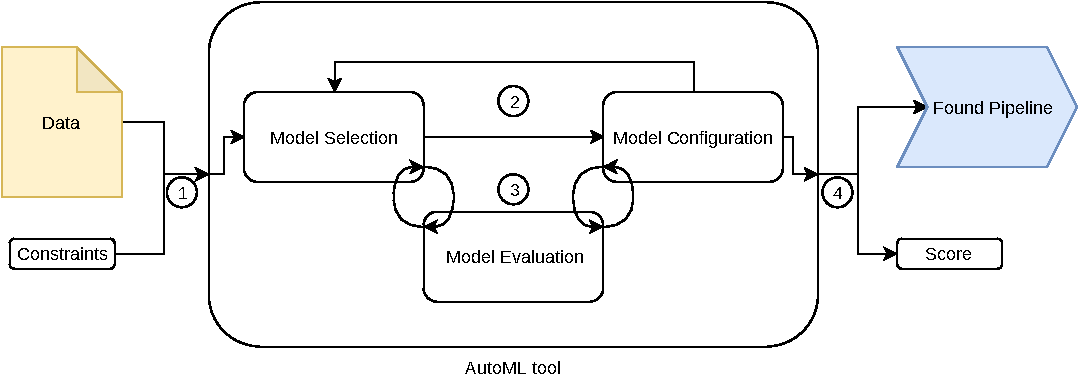
\includegraphics[width=\textwidth]{gfx/Figures/Theory/AutoMLTool.pdf}
    \caption{High level view of a conceptual AutoML tool. }
	\label{fig:theory:conceptualAutoMLTool}
\end{figure}
The general workflow of an AutoML tool is also numbered and illustrated in the figure and can be generalized with the following steps:
\begin{enumerate}
    \item AutoML tool gets input data and some execution constraints as an input.
    \item Model selection and model configuration are repeated until execution constraints are met.
    \item Model selection as well as model configuration can perform a model evaluation to get a score for any pipeline candidate they encounter.
    \item After the constraints are met, the best found pipeline as well as the score of this pipeline are given as an output.
\end{enumerate}
The model evaluation step is usually performed by training a pipeline on one big portion of the input data and testing it with a smaller portion of the data, sometimes called validation data, while measuring some kind of performance measurement, for example the accuracy of predictions or some error metric.
But other evaluation techniques for example like a Cross-Validation are also common.\newline
While the model evaluation step is only very loosely defined and usually not a complex procedure, the model Selection and model configuration steps of the AutoML workflow are more sophisticated.
They have to select a suitable candidate from a usually large space. 
Both spaces, for model selection as well as for model configuration, will be individually explained in the following.

\subsection{Model Selection}
\label{sec:theory:automl:selection}
Model selection is the task of selecting $1$ to $n$ components that will be part of the machine learning pipeline and sequentially traversed when data is passed through the pipeline.
For example, a valid pipeline would be to apply a Principal-Component-Analysis on the data as a first component and to use a Support Vector Machine for classification on the processed data as a second component afterwards.
In this step of the workflow, the space one candidate has to be selected from, consists of all this valid pipeline, which usually have two or more components.\newline
Usually there are three types of components:
\begin{itemize}
    \item Pre-Processing: Transform the input data before presenting it to the learning model.
    \item Learning Model: Perform the actual machine learning task on the data, for example classify a datapoint after training.
    \item Post-Processing: Transform the output of the learning model before yielding it as a final result.
\end{itemize}
Although in theory only a single learning model is necessary and components for pre- and post-processing are optional, at least pre-processing is very common in machine learning pipelines and included most of the time.\newline
It is possible to use more than one component from each type in a single pipeline and pipelines with arbitrary complexity can be created.
More than one pre- or post-processor can be used in sequence or in parallel with some kind of aggregator subsequently.
Equally, more than one learning model can be combined to be used as a composite model with a proper aggregation method like for example Bagging of models~\cite{Breiman-BaggingPredictors}.
An example for such a more complex pipeline is illustrated in figure~\ref{fig:theory:complexPipeline}.\newline
\begin{figure}[ht!]
    \centering
    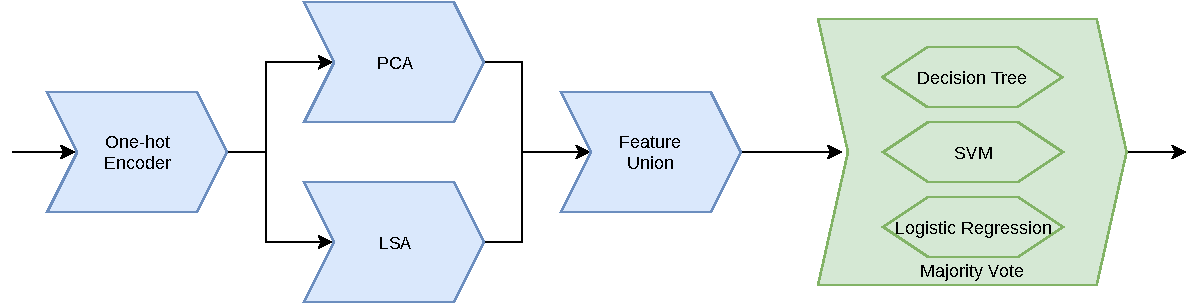
\includegraphics[width=\textwidth]{gfx/Figures/Theory/ComplexPipeline.pdf}
    \caption{Example for a more complex pipeline with four pre-processing components in blue: A One-hot Encoder, a Feature Union of a PCA and a LSA. The learning model in green is a Majority Voter as an aggregation of a Decision Tree, a SVM and a Logistic Regression Classifier. }
	\label{fig:theory:complexPipeline}
\end{figure}
Model selection, where the resulting pipelines can have this complexity, needs to add a structural relationship between the pipeline components to the selected components.
Therewith, model selection can be written as simple formalization with two things:
\begin{itemize}
    \item For all possible components $C=\{c_1, ..., c_n\}$ a $C' \subseteq C$ of components that will be used to construct the pipeline.
    \item A binary relation $\prec$ over $C'$ that defines which component is a data input for another component to define an order of the components for the pipeline as well as aggregation of several components with one component. 
\end{itemize}
Nevertheless, to find a valid set $C' \subseteq C$ is not a trivial task.
For example, when an aggregator for multiple parallel pre-processing components is needed, a valid choice could be a Feature Union component but a Decision Tree component would be invalid for this pipeline position.
Therefore, if the pipelines shall be allowed to be more complex than for example a single pre-processing component and a single learning model, there is a big set of constraints for valid subsets of the candidate space of the model selection $C$.

\subsection{Model Configuration}
\label{sec:theory:automl:configuration}
With the resulting component set after the model selection step selected its candidate $C'=\{c_1, ..., c_r\}$ the pipeline is not ready to be used yet.
Usually each component of $c_k \in C'$ has a set of hyperparameter and for each one a concrete value is needed.
Therewith, the candidate space for the model configuration step is dependent on the resulting candidate from the model selection step.
Each component $c_k$ has a set of hyperparameter $\Theta_k=\{ \theta_{k,1}, ..., \theta_{k,j} \}$ where each hyperparameter has a range where the value for this hyperparameter has to be chosen from.
Such a range can for example be a numeric set $\mathbb{N}$ or a custom set like for example $\{\textrm{true}, \textrm{false}\}$.\newline
When combining all ranges $\bigcup\limits_{i=1}^r \Theta_i$ a parametrization space with dimension $r$ is defined as the candidate space for the model configuration step, where configuration vectors can be drawn.
An example for a concrete parametrization drawn from a three dimensional parameter space is shown in figure~\ref{fig:theory:parameterSpace}
\begin{figure}[ht!]
    \centering
    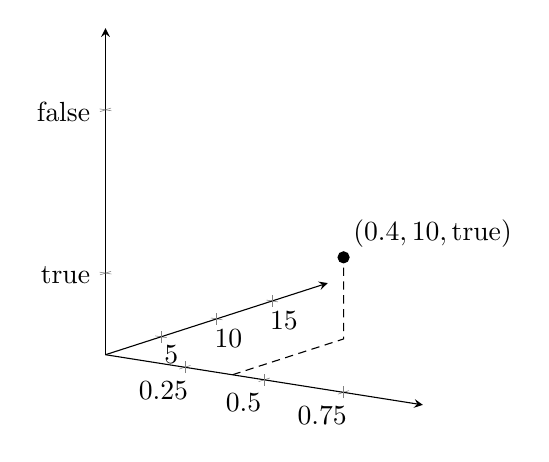
\begin{tikzpicture}
        \begin{axis}[
          view={35}{15},
          axis lines=center,
          xtick={0.25, 0.5, 0.75},ytick={5,10, 15},ztick={-10,-5,5,10},
          xmin=0,xmax=1,ymin=0,ymax=20,zmin=0.5,zmax=2.5,
          zticklabels={true, false},ztick={1,2},
          z tick label style={anchor=east}]
        ]
        \addplot3 [only marks] coordinates {(0.4,10,1)};
        \addplot3 [no marks,densely dashed] coordinates { (0.4,0,0.5) (0.4,10,0.5) (0.4,10,1)};
        \node [above right] at (axis cs:0.4,10,1) {$(0.4,10,\textrm{true})$};
        \end{axis}
    \end{tikzpicture}
    \caption{A parameter configuration with the values $(0.4,10,\textrm{true})$ inside the parameter space with the dimensions $[0..20]$, $[0, 1)$ and $\{\textrm{true}, \textrm{false}\}$ }
	\label{fig:theory:parameterSpace}
\end{figure}
Each of this vectors is a valid candidate and will result in a working pipeline instance created from $C'$ and configured with this vector.
When such a pipeline is constructed and configured with the vector values it can finally be evaluated as a candidate pipeline.

\subsection{Formalization of AutoML as an Optimization Problem}
\label{sec:theory:automl:optimization}
The choices in the model selection and model configuration step for one candidate out of the corresponding candidate spaces should not be arbitrary.
Evaluations of a candidate pipeline yield a score for this candidate and intuitively a suitable AutoML approach should try to select candidates with scores as good as possible.
Therefore, the AutoML problem is often considered as a special form of an optimization problem and can be formalized as one as well.\newline
\textcite{Feurer-Cash} give a formalization for AutoML problems as a so called \textit{Combined Algorithm Selection and Hyperparameter optimization} problem, or short \textit{CASH} problem.
Their definition is the following:
\begin{equation*}
    A^*, \lambda_* \in \> \underset{A^{(j)} \in \mathcal{A},\lambda \in \Lambda^{(j)}}{\mathrm{argmin}} \> \frac{1}{K} \sum_{i=0}^K \mathcal{L} (A_\lambda^{(j)}, D_{\textit{train}}^{(i)}, D_{\textit{valid}}^{(i)})
\end{equation*}
This formula consists out of the following parts:
\begin{itemize}
    \item $A^*$: The best solution of the algorithm selection, i.e. for the AutoML setting the best pipeline construction found in the model selection step
    \item $\lambda_*$: The best hyperparameter configuration for $A^*$ found in the hyperparameter optimization step, i.e. the model configuration step for AutoML
    \item $\mathcal{A}$: A set of possible algorithms to choose from and given in the form $\mathcal{A} = \{A^{1}, ..., A^{R} \}$, which is the set of all valid pipeline component combinations in the case of AutoML
    \item $\Lambda^{(j)}$: Each algorithm $A^{(j)} \in \mathcal{A}$ has a parameter configuration domain $\Lambda^{(j)}$, where a concrete parametrization $\lambda$ can be selected out of
    \item $\frac{1}{K} \sum_{i=0}^K $: This is used to calculate the K-fold cross-validation of a pipeline, but other evaluation metrics are also possible if the formula is adjusted accordingly
    \item $\mathcal{L} (A_\lambda^{(j)}, D_{\textit{train}}^{(i)}, D_{\textit{valid}}^{(i)})$: Is the loss, calculated with the loss function $\mathcal{L}$, of the algorithm $A^{(j)}$ configured with the parametrization $\lambda$, trained on the $i$-th split of the training data $D_{\textit{train}}^{(i)}$ and evaluated on the validation data $D_{\textit{valid}}^{(i)}$
\end{itemize}
In summary, the goal is to select an algorithm and a parameter configuration for this algorithm, such that the cross-validation loss for a for a given training and validation set is minimal.

\section{Black Box Optimization}
\label{sec:theory:optimization}
With the formalization of AutoML as a CASH problem the question arises if it can be tackled similar to standard textbook optimization problems, where established optimization algorithms exist.
Unfortunately, the CASH problem is a special case of optimization problem called \textit{Black Box} optimization problem.\newline
In the following will be explained in what way Black Box problems are different to the standard textbook optimization problem and why established optimization algorithms cannot be used.
Afterwards a selection of existing algorithms will be presented that can be used instead for the AutoML setting.
Finally, with the aid of the \textit{No-Free-Lunch Theorem}, it will be reasoned why these approaches cannot be optimal and why therefore a ensemble approach could be more promising.

\subsection{Differences to General Optimization Problems}
\label{sec:theory:optimization:differences}
\textcite{Boyd-Optimization} define a standard optimization problem as the following:
\begin{alignat*}{1}
    \underset{x}{\mathrm{minimize}} \textit{ or } \underset{x}{\mathrm{maximize}} \qquad & f_0(x)\\
    \textit{subject to} \qquad & f_i(x) \leq 0,\> i=1,...,m\\
                        &  h_j(x) \leq 0,\> j=1,...,p\\
\end{alignat*}
Here is the goal to find a value for the optimization variable $x$ such that $f_o(x)$ has either its minimum or maximum value.
Hereby, $x$ does not have to be a single value but can be a vector of values in the case of a multi-objective optimization problem.
$f_0$ is usually called a objective function or cost function.
The choices for $x$ can be limited by a set of inequality constraint functions $g_k$ and a set of equality constraint functions $h_i$.
If $m=p=0$, there are no constraint functions and the optimization problem is called unconstrained.
For such cases, x could be any value from the domain of $f_o$.\newline
If $f_0$ has certain properties, for example if it is convex, there are specialized optimization methods that can solve the optimization problem without the derivative $f_0'$.
But for general optimization algorithms, where no properties of $f_0$ besides derivability are expected, $f_0'$ is required to solve the optimization problem analytically.\newline
The problem is, for some optimization problems the exact formula of $f_0$ is not known or not given and therefore no derivative can be calculated such that the general optimization algorithms are not applicable.
Instead, it is only possible to obtain $f_0(x)$ for any requested $x$ for example by looking it up in a table or asking an expert.
For such problems it is only possible to observe the inputs and corresponding outputs of $f_0$ but the inner workings are hidden.
$f_0$ is metaphorically a black box, where something goes in and something comes out but it is not possible to look inside, and therefore such optimization problems are called Black Box optimization problems.\newline
AutoML, considered as a CASH problem, is a Black Box optimization problem as well.
It is not possible, or at least not yet realizable, to determine a general formula for $f_0$.
The relationship between the properties of the dataset, the different pipeline components with their configuration parameters and other factors, as for example randomness of some components, is way to complex and inscrutable to be formulated into a single cohesive function.
But it is possible to to get a evaluation of a $x$, i.e. a concrete pipeline with a complete configuration, by training and testing the pipeline with given data and a evaluation metric like for example a cross-validation.
The absence of a concrete formula for $f_0$ but the possibility to determine $f_0(x)$ renders AutoML as a Black Box optimization problem.\newline
Without the possibility to determine a optimal or near optimal candidate analytically, in the case of a Black Box optimization problem a series of candidates has to be selected and evaluated while trying to find or at least approximate a optimal solution.
Now the question remains for the AutoML setting how candidates from the two presumably large candidate spaces of model selection and model configuration should be selected for each iteration and how such a approximation can be attempted.\newline
A solely random selection in every iteration is not very likely to find good results with such a high number of choices.
Since the approach evaluates several candidates iteratively, a better approach would be to base the selection on knowledge gathered from previous iterations.\newline
Several algorithms were developed to tackle such a iteratively approximation of the optimum of a Black Box optimization problem.
Some of them have already showed promising results for AutoML CASH problems and therefore the current state-of-the-art AutoML research works primarily with the following three optimization strategies:
\begin{itemize}
    \item (Heuristic) Search
    \item Genetic and Evolutionary Algorithms
    \item Bayesian Optimization
\end{itemize}
In general is every Black Box optimization strategy defined by a selection of candidates out of the candidate space that will is evaluated and an order in which they are evaluated.
Hereby, the selection as well as the order can be defined in many ways.
For example it could be partially or fully pre-defined or random.
Also it could be defined implicitly and other selected candidates and their order can depend on the knowledge gathered from the evaluation of one candidate.\newline
For each one of the aforementioned Black-Box optimization strategies this candidate selection and candidate order will be explained in general and on the basis of some concrete algorithms, which were used in the AutoML research.
These explanations of the strategies will be supported with a simple running example.
The unconstrained target function $f_0 \left( \begin{bmatrix}x\\y \end{bmatrix} \right) = x^2 + y^2$, which can be seen in figure~\ref{fig:theory:target-function}, shall be minimized.
This function is defined in $\mathbb{R}^2$ and has one global minimum.
\begin{figure}[ht!]
    \centering
    \begin{subfigure}{0.48\textwidth}
        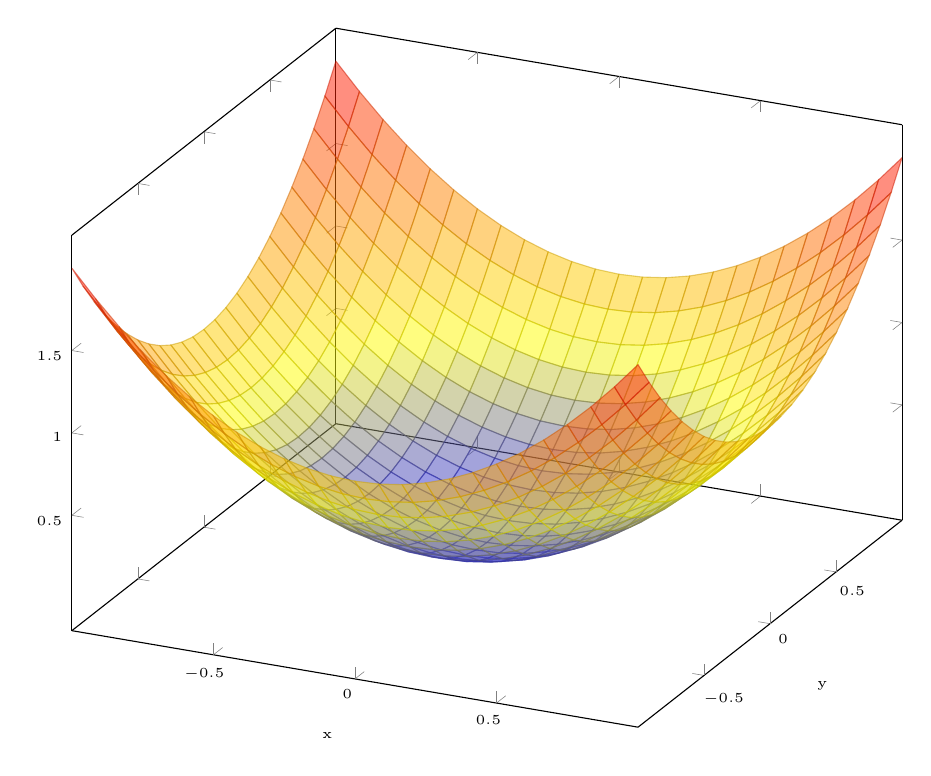
\begin{tikzpicture}
            \begin{axis}[
                xmin=-1,xmax=1,ymin=-1,ymax=1,
                width=\textwidth,
                xlabel = {x},
                ylabel = {y},
                xtick = {-0.5,0,0.5},
                ytick = {-0.5,0,0.5},
                ztick = {0.5,1,1.5},
                tick label style={font=\tiny},
                label style={font=\tiny}
            ]
                \addplot3[
                    surf,
                    opacity=0.5,
                    samples=25, samples y=25,
                    domain=-1:1, domain y=-1:1
                ]
                {x^2+y^2};
            \end{axis}
        \end{tikzpicture}
    \end{subfigure}
    \begin{subfigure}{0.48\textwidth}
        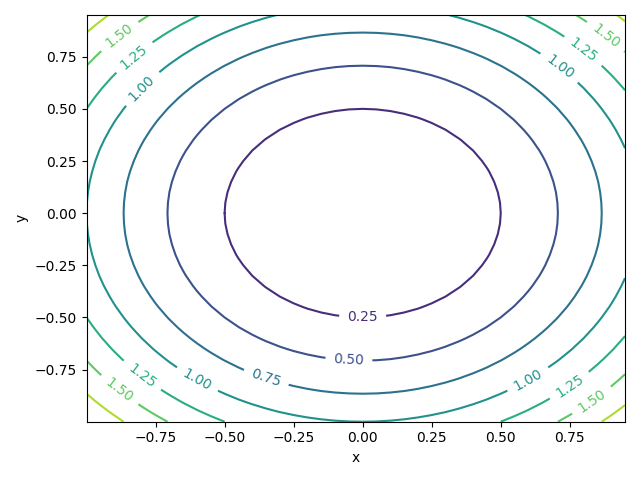
\includegraphics[width=\textwidth]{gfx/Figures/Theory/OptimizationTargetFunctionContour.png}
    \end{subfigure}
    \caption[.]{A two dimensional target function with a global minimum at \ensuremath{\begin{bmatrix} 0\\0 \end{bmatrix}}. On the right as a surface plot and on the left as a contour plot.}
    \label{fig:theory:target-function}
\end{figure}

\subsection{Optimization by Searching}
\label{sec:theory:optimization:search}
Optimizing with a search will evaluate candidates with the concept of \textit{Neighborhood} between candidates.
Starting with a single starting candidate, the search will extend its set of evaluated candidates by evaluating a neighboring candidate of one candidate out of this set.
The concrete definition of this neighborhood concept is depending of the examined search space, modelled out of the candidate space, and the applied search algorithm.
For example, a neighbor could be any candidate within a certain distance of another candidate or a graph could be created out of a set of candidates and neighbors of a candidate are the adjacent candidate nodes in the graph.
Which neighbor should be selected for evaluation next, therefore defining the order of candidate evaluations implicitly, can vary with the different approaches as well.
It could be completely random, pre-defined before the search starts or based on a heuristic scoring of the candidates.\newline
A wide range of search algorithms were developed in the corresponding research area and the most of them are applicable for optimization problems as well with a suitable neighborhood concept.
Some search algorithms are used in state-of the art AutoML approaches and three of them are explained in more detail with the aid of the running example in the following.


\textbf{Random Search}: The Random Search Algorithm comes in two variants.
In the first one the candidates are completely drawn randomly out of the whole candidate space and evaluated.
When the optimization budget is spent, the best candidate is returned as the result.
Since this method does not use any knowledge gathered during the optimization, it depends on luck and the optimization budget if the optimal solution or at least a near optimal solution is found.\newline
In the second one, a starting candidate is drawn at random out of the candidate space and evaluated.
The next candidate will be randomly drawn out of a hypersphere with a pre-defined radius around the starting candidate and evaluated.
If the drawn candidate has a better evaluation score than the starting candidate, the next candidate will be drawn from a hypersphere around the second candidate and from the hypersphere of the starting candidate otherwise.
This loop is continued until the optimization budget is spent. Since this method is very prone to local minima/maxima, it is a possible improvement to remember the current best candidate, select a new completely random start point and start the loop over, if there was no improvement in the last $n$ iterations of the current loop.
Both variants are illustrated for the running example in figure~\ref{fig:theory:random-search}.\newline
One example of the Random Search algorithm applied in the context of AutoML is the \textit{Hyperband} approach~\cite{Li-Hyperband}.
Here, multiple parallel working instances of Random Searches are evaluating candidates in a joint space of model selection and model configuration to cover as much of the candidate space as possible.
The initial problem is that multiple instances combined require a big portion of the optimization budget.
This was tackled by treating each random search as the arm of the bandit and canceling single search instances over time that do not find candidates with high evaluation scores and which therefore probably have a low regret.
By terminating some probably low performing searches the optimization budget can be spent on mor promising search instances.
Strategies like this are often referred to as \textit{Early Stopping}.
In the context of Hyperband, selecting the search instances which will not be stopped early is done in a non-stochastic manner with the \textit{Successive Halving} algorithm~\cite{Jamieson-SuccessiveHalving}.
\begin{figure}[ht!]
    \centering
    \begin{subfigure}{0.48\textwidth}
        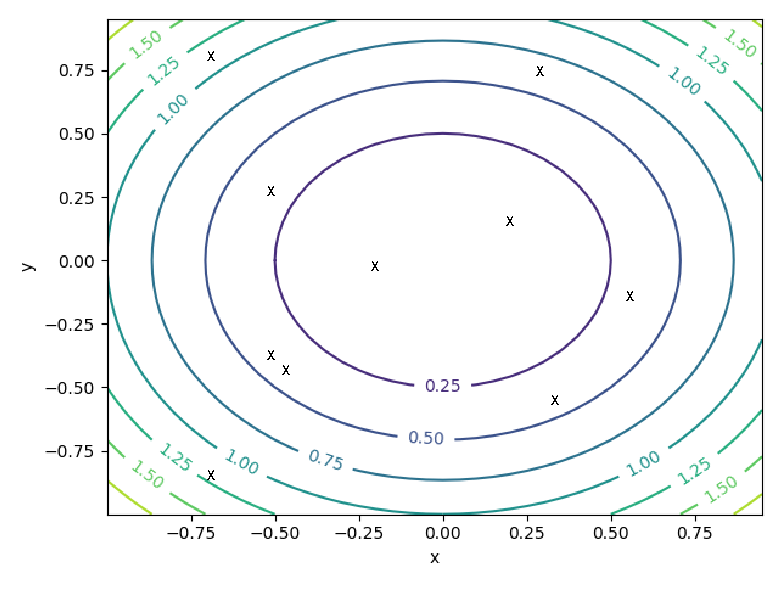
\includegraphics[width=\textwidth]{gfx/Figures/Theory/RandomSearch.pdf}
    \end{subfigure}
    \begin{subfigure}{0.48\textwidth}
        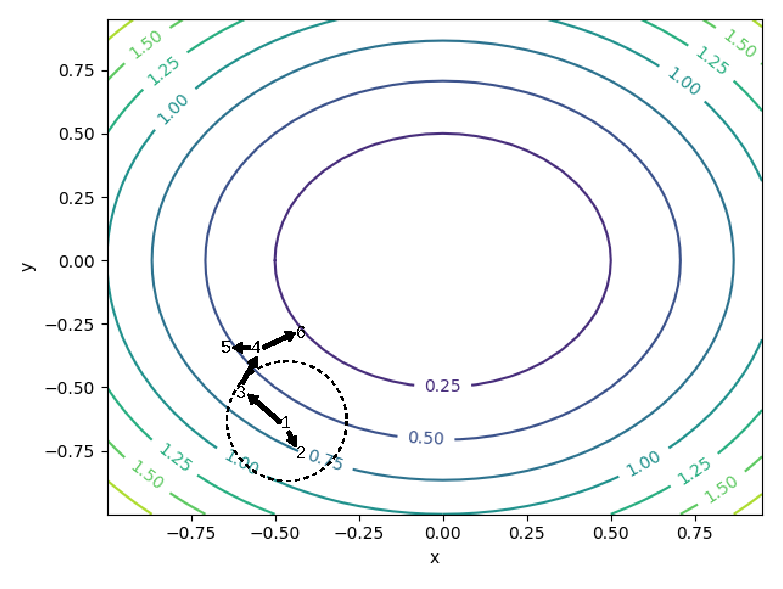
\includegraphics[width=\textwidth]{gfx/Figures/Theory/RandomSearchHypersphere.pdf}
    \end{subfigure}
    \caption{On the left is the first variant with a few randomly selected candidates. On the right are six possible first iterations of the second variant. The hypersphere is only shown for the first candidate.}
    \label{fig:theory:random-search}
\end{figure}


\textbf{Grid Search}: A Grid Search tries to cover with a na\"ive brute-force approach as much of the candidate space as possible.
From each dimension of the candidate space a few values are selected either manual, or more commonly by selecting values from the dimensions allowed range in periodic intervals.
For example, if the x-dimension of the running example should be evaluated in the range $[-1,1]$, depending on the available optimization, potential value selections for this dimension could be $\{-1,0,1\}$ or $\{-0.75,-0.25,0.25,0.75\}$.
With this method the candidate space is discretized and therewith becomes enumerable.\newline
After selecting the value sets for each dimension, the Cartesian product of all sets is calculated.
The elements of this Cartesian product, which are valid candidates because they have a value of each dimension, are the candidates that will be evaluated during the search and for the order of evaluations any arbitrary sequence of the sets elements can be selected.
After either all candidates from the Cartesian product are evaluated or if the optimization budget is spent, the best evaluated candidate is the overall optimization result.
An illustration of a Grid Search over the candidate space of the running example can be seen in figure~\ref{fig:theory:grid-search}.\newline
Therefore, as opposed to Random Searches where by chance only a small portion of the candidate space could be covered, a certain coverage of the space is assured.
Especially in contrast to the second variant of the Random Search, the advantage is that there is no risk of getting stuck in a local optimum.
But im comparison of with the second Random Search variant the main drawback of a Grid Search comes clear, i.e. a Grid Search does not utilize the knowledge gathered from previous evaluations at all, since the evaluation order is completely predefined.
This, even if the Grid Search would evaluate a candidate comparably close to a global optimum, it would completely disregard this chance and not continue the search closely to this candidate to potentially find this global optimum.\newline
Grid Searches are as well as Random Searches classical algorithm choices for Hyperparameter optimization because they are easy to implement and very resource-efficient due to their simplicity such that a high number of candidate evaluation can be performed.
In the context of AutoML, a 2-dimensional Grid Search was utilized in the Weka toolbox~\cite{Witten-Weka} for a simple AutoML approach.
There, a joint candidate space was searched with a set of classifiers for model selection on one dimension and the other dimension is used to select the amount of components of Partial Least Squares filter, which is used as a pre-processor, and can therefore be considered as a simple model configuration.
\begin{figure}[ht!]
    \centering
    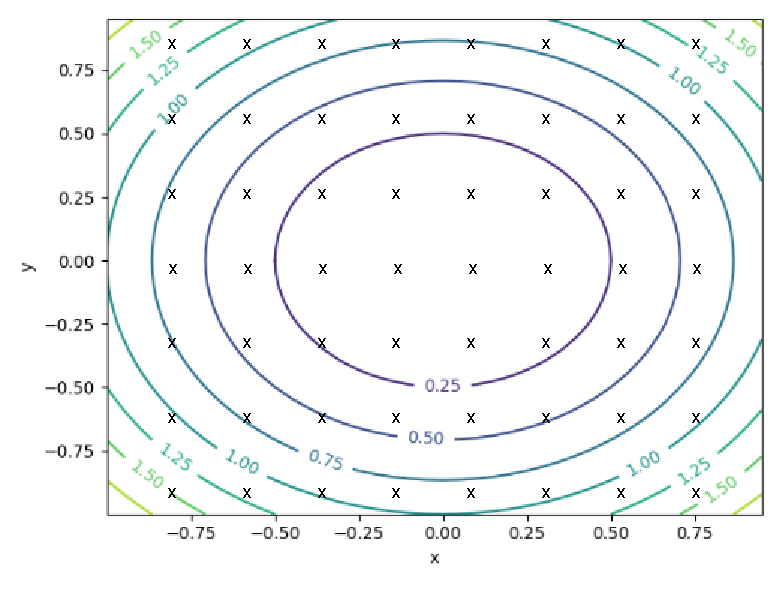
\includegraphics[width=\textwidth]{gfx/Figures/Theory/GridSearch.pdf}
    \caption{Illustration of a Grid Search covering the search space of the running example systematically.}
    \label{fig:theory:grid-search}
\end{figure}


\textbf{(Heuristic) Graph Search}: While a Random Search does it partially leaf to chances which candidates are evaluated, the candidate space will not be adequately covered with a high probability, a Grid Search will have certain coverage guarantees by default.
On the other hand, a Grid Search will not utilize any gathered knowledge about the candidate space while at least the second variant of a Random Search is capable of utilizing knowledge about one prior evaluation.
A Graph Search, usually in combination with a heuristic for search guidance, tries to achieve a trade-off between the advantages of both other presented search algorithms, i.e. having a solid coverage of the candidate space as well as utilizing knowledge gathered during the search.\newline
As the name suggests, for a Graph Search the candidate space is depicted as a graph, but how the space is transformed into a representation consisting out of nodes and edges is very domain and approach specific and several methods exist.
For example, each node could represent a concrete candidate out of the space and can be directly evaluated.
The edges would connect such candidate nodes, if they have a maximum distance to each other, comparable to the hyperspheres the second Random Search variant uses to define neighborhood.
Another method could be to use a tree as a search graph, where only the leaf nodes are concrete candidate nodes, which can be evaluated.
Here, the inner nodes are used to progressively discretize the candidate spaces dimensions in a hierarchical manner by splitting the range into multiple intervals and creating a new child node for each one.
This is continued until the intervals of each dimension either only consist of one element or are small enough such that one value out of it can be selected arbitrarily.
At this point, a leaf node would be the child node because for each dimension a value is selected such that the candidates configuration is complete and could be evaluated.\newline
With a given start node and a method to expand this start node incrementally into a bigger graph, a large amount of search algorithms exists to utilize to search this graph for the best candidate.
They mostly differ in the selection method which unexplored node should be visited next.
The set of nodes, consisting of the unexplored neighbors of already visited and expanded nodes is called a \textit{Search Front} and it is exemplarily illustrated for a search tree in figure~\ref{fig:theory:graph-search-front}.
\begin{figure}[ht!]
    \centering
    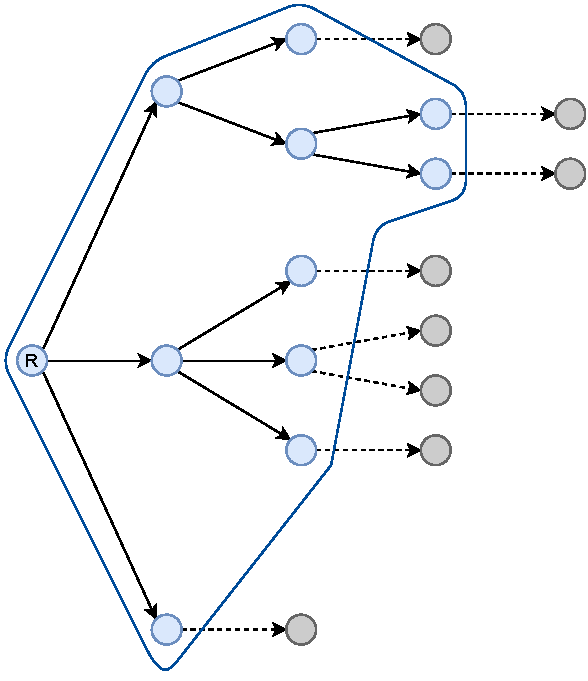
\includegraphics[width=\textwidth]{gfx/Figures/Theory/GraphSearchFront.pdf}
    \caption{After a few iterations of a search algorithm beginning at the root node, a few nodes are already explored and expanded, here illustrated in blue. The expanded child nodes of the searched area(blue) are the search front(grey nodes) and one of them will be explored and expanded in the next search iteration.}
    \label{fig:theory:graph-search-front}
\end{figure}
Some search algorithms select nodes out of the search front  based on the point in time, where they were added to the search front, like for example a Depth-First Search or a Breadth-First Search.
This is a valid approach if the optimization budget is very large and is sufficient to traverse the graph more or less completely.
But in the most use-cases the budget will not even be remotely sufficient for this and the next node out of the search front should be the node, were the best evaluation score or a path to the best evaluation score can be expected.\newline
In the case of the first described method to transform a candidate space into a graph, where each node is a candidate and can be evaluated, this is trivial.
But for the second method, this is more challenging because only leaf nodes can be evaluated and inner nodes not.
To assign a score to a inner node without searching the complete sub-graph below it, an estimation method is utilized, usually called a heuristic.\newline
For example with some available domain knowledge, if certain discretization intervals or selected values are more promising than other, the heuristic can assign higher scores to the corresponding child nodes representing the interval or value.
In the AutoML context this could be done, if for example a certain pipeline component performed outstandingly for previous experiments with this component.
But usually this will not be the case because the relationships between pipeline components to each other and their parameter configuration is too complex and even minor changes can have a big influence to the evaluation score.
Therefore, it is hard to score an incomplete pipeline even with pre-existing domain knowledge.\newline
Without a way to deterministically score a inner node, a probabilistic approach is more promising.
Here, it can be assumed if enough leaf nodes at the end of the sub-graph below the inner node, which shall be scored, are evaluated, it is possible to score the inner node based on these evaluations with a sufficient certainty.
Which path to follow to reach a leaf node in the sub-graph is decided randomly.
To score something based on a a series of random experiments is called a \textit{Monte-Carlo} simulation/experiment and is a common approach to obtain a value, where the exact calculation of the value is either impossible or too complex.
This combination of utilizing a heuristic Graph Search with Monte-Carlo simulations as a heuristic for optimization in the AutoML context was applied to a Best-First Search in the ML-Plan approach~\cite{Mohr-ML-Plan}.

\subsection{Genetic and Evolutionary Optimization}
\label{sec:theory:optimization:genetic}
Genetic and Evolutionary optimization methods try to transfer the process of the evolution in nature, as described in Charles Darwins \textit{Natural Selection} theory, to computational optimization.
Exactly like an biological evolution model for a species, the optimization process is modelled in consecutive generations and each generation consists out of a high number of individuals.
Ideally, only the individuals which are best adopted to their surroundings should produce offsprings and therefore create a succeeding generation, which is based on this individuals with minor changes.
This is often referred to as \textit{Survival of the fittest}.
Transferred to optimization, this would mean that each individual is a possible solution candidate and therefore a generation is a set of solution candidates.
Starting with a base generation of usually randomly created individuals, a Genetic Algorithm follows the following pattern:
\begin{enumerate}
    \item Evaluate each individual of the current generation.
    \item Select a subset of the current generation that will be used to create the next generation. Normally, this subset is created as a mix of the highest scoring individuals as well as some randomly selected individuals to prevent focussing on local optimums. But other selection approaches were also developed.
    \item Generate the next generation with the selected subset. A pre-defined ratio of individuals will be directly copied into the next generation and the remaining individuals will be modified with evolutionary operators to attempt an enhancement.
\end{enumerate}
This steps are usually repeated until either a certain target score is achieved with one individual, the optimization budget is spent or the scores did not improve over the last $n$ generations.\newline
The aforementioned evolutionary operators work on so called \textit{genetic representations} of candidates, sometimes also called \textit{Genomes} or \textit{Chromosomes}.
In theory nearly every data structure is a suitable for this representation but most often are simple arrays or vectors used, where each cell represents one property of the candidates or alternatively one dimension of the candidate space.
For the running example this would mean an array with length 2, one for the $x$ and one for the $y$ dimension.\newline
Just as in the general principle from biological evolution, these genomes can change by random mutations as well as by recombination, when two individuals produce a new individual.
For a mutation, one individual is selected and one or more cells are changed slightly at random and the other values are kept the same.
If the amount of cells to change is not pre-defined, this is the same idea of randomly selecting a candidate out of hypersphere around another candidate already mentioned for Random Searches.
Thus, if the only applied evolutionary operator is the mutation operator, a Genetic Algorithm would be conceptually comparable to multiple parallel running Random Search instances, but in combination with the recombination operator this Random Search instances can interact with each other and re-organize their current positions to increase the chance of a high candidate space coverage.\newline
A recombination based on two genomes $g_1$ and $g_2$ to produce a new genome $g^*$ is usually performed as a cross-over.
For each cell of $g^*$ the value is taken from either $g_1$ or $g_2$.
Depending on the type of cross-over, there $k \in [1 ... |g^*| - 1]$ cross-over points, which are selected randomly.
Each cross-over point marks an index of $g^*$ at which it will be switched from $g_1$ to $g_2$ or vice versa from which source genome the next value will be taken from.
An example for a two-point cross-over is shown in figure~\ref{fig:theory:crossover}.
\begin{figure}[ht!]
    \centering
    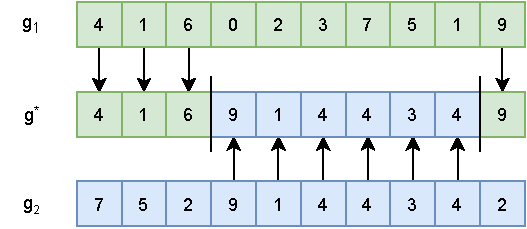
\includegraphics[width=\textwidth]{gfx/Figures/Theory/Crossover.pdf}
    \caption{An example of a two-point cross-over to produce $g^*$ from $g_1$ and $g_2$.}
    \label{fig:theory:crossover}
\end{figure}
With the random factors during selecting the individuals for the generation of the next generation as well as during the application of the evolutionary operators, Genetic and Evolutionary optimization approaches are a stochastic optimization method just as a Random Search or certain Graph Search algorithms and heuristics.
Therefore, the chances of finding a high scoring solution, the coverage of the candidate space as well as the risk of ending in a local optimum are highly dependent on the number of iterations the algorithm performs as well as other configuration parameters like for example the size of each generation.\newline
Additionally to the challenges of handling chances and probabilities emerging from any probabilistic approach, in the context of AutoML there is one more major challenge in applying a Genetic Algorithm for optimization.
A more complicated data structure is needed to represent a pipeline configuration as a single genome because usually they do not have a maximal length and can be composed as a arbitrary graph or tree, which can not represented in an array.
Even if a suitable data structure is found, the mutation and cross-over implementations have to be made very cautious, because representations of pipelines can be very error-prone.
Already small changes to one representation value can lead to an invalid pipeline constructions which cannot be instantiated.\newline
Two state-of-the-art approaches tackling this challenges and applying Genetic Algorithms as optimizers for AutoML problems are \textit{TPOT}~\cite{Olson-Tpot}, using expression trees as a data structure, and \textit{RECIPE}~\cite{Guimar-Recipe}, using grammar-based genetic programming.

\subsection{Bayesian Optimization}
\label{sec:theory:optimization:bayesian}
From all the aforementioned optimization methods, Bayesian optimization utilizes the knowledge from previous candidate evaluations the most.
The goal is to select the most promising candidate for the next evaluation and therefore minimize the overall amount of evaluations until a near-optimal score is reached.
Since each evaluation in the context of AutoML comes with assembling a candidate pipeline and usually performing a cross-validation of the pipeline on the dataset, each evaluation consumes a lot optimization budget.
Therewith, Bayesian Optimization is one of the most used Black Box optimization approaches in recent AutoML research.\newline
The notation of a \textit{most promising} candidate could be interpreted in different ways.
For example, a candidate near the current optimum, which has a high probability of having a comparable or even better score, or a candidate in a completely unevaluated region of the candidate space, where therefore a optimum could lie unnoticed.
But in the case of Bayesian Optimization, this notation of most promising is more sophisticated.\newline
In general, the goal is to create with Bayesian statistics a surrogate function model that replicates the unknown target function as closely as possible.
To model the Bayesian surrogate a common choice is a regression based on a Gaussian Process.
Detailed information about Gaussian Processes can be found for example in~\cite{Rasmussen-Gaussian-Processes}.\newline
This surrogate is based on several evaluations as samples and will become more precise with each new sample, which is usually the next most promising candidate.
For the actual selection of the next most promising candidate sample, a so called \textit{Acquisition Function} is used and the next value will be at an optimum of this acquisition function.
The value of such an acquisition function for a candidate are based on two factors:
\begin{enumerate}
    \item The estimated score of the candidate based on the modelled Bayesian surrogate.
    \item The size of the credible interval of the Bayesian surrogate model at the position of the candidate.
\end{enumerate}
The size of the credible interval is especially important, because if at a point this interval is very broad, the chances are higher that the value of the target function can differ widely from the surrogate at this position.
Of course it can differ in both directions but this can be examined with an additional sample at this position.
Therefore, if the estimated value already indicates an optimum and additionally the credible interval is broad, the value of the target function could be even more optimal at this position and it is the most promising candidate to be drawn as the next sample.
For candidates that were already evaluated, this acquisition score is set to zero because the target score at this position is already known and the surrogate can be certain at this position.
A graphical intuition for the concept of acquisition functions is given in figure~\ref{fig:theory:acquisition-function}, where Bayesian optimization on one dimension of the running example is illustrated.
\begin{figure}[ht!]
    \centering
    \begin{subfigure}{\textwidth}
        \centering
        \begin{tikzpicture}
            \begin{axis}[
                xmin=-1, xmax=1,
                ymin=0, ymax=1,
                domain=-1:1,
                xlabel=$x$,
                ylabel=$f_0 \left( \begin{bmatrix}x\\0 \end{bmatrix} \right) $,
                no markers,
                height=5cm,
                width=0.75\textwidth,
            ]
                \addplot[lime]{x^2};
            \end{axis}
        \end{tikzpicture}
        \caption[.]{Slice of the target function $f_0$ at $y=0$.}
    \end{subfigure}
    \begin{subfigure}{\textwidth}
        \centering
        \begin{tikzpicture}
            \begin{axis}[
                xmin=-1, xmax=1,
                ymin=-0.2, ymax=1,
                domain=-1:1,
                xlabel=$x$,
                ylabel=$f_s \left( \begin{bmatrix}x\\0 \end{bmatrix} \right) $,
                height=5cm,
                width=0.75\textwidth,
            ]
                \addplot [only marks,red] coordinates {(-0.7,0.49) (-0.5,0.25) (-0.2,0.04) (0.4,0.16) (0.85,0.7225)};
                \addplot [,
                    smooth,
                    no marks,
                    solid,
                    line join = round,
                    red
                ] coordinates {(-1,0.875) (-0.7,0.49) (-0.5,0.25) (-0.2,0.04) (0.1,0.05) (0.4,0.16) (0.7,0.5) (0.85,0.7225) (1,0.9)};
                \addplot [,
                    smooth,
                    no marks,
                    dashed,
                    line join = round,
                    red
                ] coordinates {(-1,0.675) (-0.85,0.58) (-0.7,0.49) (-0.56,0.46) (-0.5,0.25) (-0.4,0.05) (-0.2,0.04) (0.1,0.2) (0.4,0.16) (0.7,0.29) (0.85,0.7225) (1,0.99)};
                \addplot [,
                    smooth,
                    no marks,
                    dashed,
                    line join = round,
                    red
                ] coordinates {(-1,1.075) (-0.85,0.79) (-0.7,0.49) (-0.64,0.31) (-0.5,0.25) (-0.35,0.21) (-0.2,0.04) (0.1,-0.11) (0.4,0.16) (0.55,0.58) (0.85,0.7225) (1,0.81)};
            \end{axis}
        \end{tikzpicture}
        \caption[.]{
            Estimated surrogate function $f_s$ modelled after 5 samples.
            The evaluated samples are shown as red dots, the surrogate function as a red line and the credible intervals as the two red dashed lines.
            Important note: The values of the surrogate function and the credible intervals are not actually calculated but are only rough estimates to give an intuition of the method.
        }
    \end{subfigure}
    \begin{subfigure}{\textwidth}
        \centering
        \begin{tikzpicture}
            \begin{axis}[
                xmin=-1, xmax=1,
                ymin=-0.5, ymax=0.1,
                domain=-1:1,
                xlabel=$x$,
                ylabel=$f_a \left( \begin{bmatrix}x\\0 \end{bmatrix} \right) $,
                height=5cm,
                width=0.75\textwidth,
            ]
                \addplot [,
                    smooth,
                    no marks,
                    solid,
                    line join = round,
                    blue
                ] coordinates {(-1,-0.1) (-0.85,-0.075) (-0.7,0)};
                \addplot [,
                    smooth,
                    no marks,
                    solid,
                    line join = round,
                    blue
                ] coordinates {(-0.7,0) (-0.6,-0.2) (-0.5,0)};
                \addplot [,
                    smooth,
                    no marks,
                    solid,
                    line join = round,
                    blue
                ] coordinates {(-0.5,0) (-0.35,-0.25) (-0.2,0)};
                \addplot [,
                    smooth,
                    no marks,
                    solid,
                    line join = round,
                    blue
                ] coordinates {(-0.2,0) (0.1,-0.4) (0.4,0)};
                \addplot [,
                    smooth,
                    no marks,
                    solid,
                    line join = round,
                    blue
                ] coordinates {(0.4,0) (0.625,-0.225) (0.85,0)};
                \addplot [,
                    smooth,
                    no marks,
                    solid,
                    line join = round,
                    blue
                ] coordinates {(0.85,0) (0.925,-0.0485) (1,-0.06)};
            \end{axis}
        \end{tikzpicture}
        \caption[.]{
            Acquisition function $f_a$ based on $f_s$ and its credible intervals after the 5 samples in.
            As in (b), the values are only estimations and not explicitly calculated.
            The minimum of $f_a$ at $x=0.1$ would be the best choice for the sixth sample.
            There the expected value of the surrogate regression is already low and the credible interval is additionally broad.
        }
    \end{subfigure}
    \caption[.]{
        Simple illustration to give an intuition of acquisition functions for the running example of minimizing $f_0 \left( \begin{bmatrix}x\\y \end{bmatrix} \right) = x^2 + y^2$.
        For simplicity will the Bayesian optimization only be used to minimize on the x-dimension and y will be set to 0, but in theory can this approach be extended to any number of dimensions.
        (a) shows a slice of the target function in green.
        (b) shows in red the already evaluated samples, the estimated surrogate function model and the credible intervals.
        (c) shows in blue the acquisition function based on the values in (b).
    }
    \label{fig:theory:acquisition-function}
\end{figure}
An exemplaric algorithm for Bayesian Optimization is given by~\textcite{Frazier-Bayesian-Optimization} with the following pseudo-code in algorithm~\ref{alg:bayesian-optimization}.
\begin{algorithm}[ht!]
    \SetAlgoLined
    Place a Gaussian process prior on $f$\;
    Observe $f$ at $n_0$ points according to an initial space-filling experimental design\;
    Set $n=n_0$\;
    \While{$n \leq N$}{
        Update posterior probability distribution on $f$ using all data\;
        Let $x_n$ be a maximizer of the acquisition function over $x$, where the acquisition function is computed using the current posterior distribution\;
        Observe $y_n = f(x_n)$\;
        Increment $n$\;
    }
    Return a solution: either the point with the largest $f(x)$, or the point with the largest posterior mean\;
    \caption{Basic pseudo-code for Bayesian optimization}
    \label{alg:bayesian-optimization}
\end{algorithm}
The functionality of this pseudo-code as well as some technical terms are explained in the following line by line:
\begin{enumerate}
    \item A probably distribution, for example a Normal distribution is selected as a initial prior distribution $f_0$ to further construct the surrogate function with.
    \item Since this initial $f_0$ is not very meaningful regarding the target function, a few candidates will be evaluated before the actual optimization loop starts.
    This candidates are selected to be a space-filling design, which means to have the best coverage of the candidate space.
    Therewith, the credible intervals between the initially observed points can be kept as small as possible before the acquisition function, which uses this intervals, is used.
    An example for a simple space-filling experiment design is to chose candidates uniformly distributed in the candidate space.
    \item Since this implementation uses the number of observations of $f$ for a given point, i.e. candidate evaluations, as a optimization budget, the variable $n$, which keeps track of the spent budget, is set to $n_0$, because this is the amount of initial evaluations.
    \item Here starts the main optimization loop.
    As long as the optimization budget is not spent and therefore $n \leq N$, further candidates can be selected and evaluated.
    \item Let $d_n$ be all evaluated points from previous iterations or from $n_0$, the surrogate function model of this iteration $f_n$ will be updated based on $d_n$.
    Therefore, a new surrogate function posterior probability distribution is calculated by updating the chosen distribution with the previous posterior distribution $f_{n-1}$ as i new prior, i.e. $f_n := f(x)|f_{n-1}$.
    \item $x_n$ is selected to be the candidate of this iteration for evaluation. It is chosen by searching the acquisition function, which was updated with the data from prior iterations, for an optimum.
    \item Get a evaluation score $y_n$ for the selected candidate of this iteration $x_n$ by observing the $f(x_n)$, thus having one more data point to base to posterior probability distribution on, to construct a more precise surrogate function $f_{n+1}$ in the next iteration.
    \item Increment $n$ because another candidate evaluation was performed and therefore the remaining optimization budget decreased.
    \item The optimization budget is spent and the main optimization loop will terminate.
    \item After the main optimization loop finishes, the algorithm will terminate and return a candidate as the result.
    It will select the best candidate among the evaluated points so far and compare it to the point with the largest posterior mean, i.e. the point where the global optimum, based on the overall constructed surrogate function $f_N$, is assumed.
    If this point is assumed better than the best evaluated candidate it will be returned and the best evaluated candidate otherwise.
\end{enumerate}
A state-of-the-art implementation of Bayesian optimization for algorithm configuration problems is \textit{SMAC}~\cite{Hutter-SMAC}, an abbreviation for Sequential Model-Based Optimization for General Algorithm Configuration.
It is utilized as an optimization approach for a joined model selection and model configuration AutoML optimization space by several approaches, including \textit{Auto-WEKA}~\cite{Thornton-AutoWeka} and \textit{auto-sklearn}~\cite{Feurer-AutoSklearn}.

\subsection{No-Free-Lunch Theorem}
\label{sec:theory:optimization:lunch}
The state-of-the-art AutoML approaches presented with their corresponding black-box optimization method have one thing in common: They all apply a single optimization algorithm to find the best candidate from a optimization space, which is a joined model selection and model configuration space.
While this is a valid approach and will found an optimal or near optimal solution for many AutoML problem instances, it is theoretically impossible that the best solution can be found with a single optimization method for every AutoML problem instance.
This can be deduced from the \textit{No-free-lunch Theorems}, which were proven for optimization problems by~\textcite{Wolpert-No-Free-Lunch-Theorems}.
In these theorems is stated that when an optimization algorithm performs superior for one problem or class of problems, it has to pay for this by performing inferior for other problems.
Of course this is only the case for optimizing with an optimization budget, because the most optimization algorithms can find the best solution if they have an unlimited budget, even if its just by simply evaluating each possible candidate.\newline
For the context of the AutoML setting, the notion of a problem class could for example be transferred to the data, which is given as an input.
Therefore, in this setting with a limited budget of time or resources, one single optimization algorithm may find the best models and configurations for some datasets but cannot achieve this for all datasets.
Thus, the presented AutoML approaches incapable of being the superior approach for all datasets.
With a given dataset $D_1$ a Genetic Algorithm may find the best solution, while a Bayesian optimization method outperforms the same Genetic Algorithm for another dateset $D_2$.\newline
It is additionally possible that the quality of an optimizer does not only depend on the input dataset, i.e. the AutoML problem class, but additionally on the concrete optimization space it operates in and the optimization budget.
This three components could be used to construct a specific problem instance for a dataset problem class.
If this optimization space is modified and thus a new problem instance $p_2$ is created from the original problem instance $p_1$, this can have a huge influence on the optimizer qualities and the optimization method that was the most successful one for $p_1$ could now theoretically be the worst one for $p_2$.\newline
Such a modification of the optimization space can be created if, for instance, the model selection part is already finished and the remaining model configuration induces the optimization space, which is now the problem of optimizing the parameters of a concrete pipeline.
Here, different optimization spaces can be created out of one initial space by pre-selecting a pipeline and different optimizers can differ in quality here as well.
For example, with a given dataset, optimizer $A$ could find good configurations for a pipeline consisting of a Principal Component Analysis followed by a Decision Tree, while optimizer $B$ does this better in the case of a single Support Vector Machine.
The same transformations of the optimization space can of course as well be done by only considering model selection instead and not model configuration.\newline
Since one optimization method will only be the best one for a limited set problem classes, it can be beneficial to use more than one optimization method together for different transformations of the optimization space to extend the set of problem classes, where these combined optimizers can be superior.\newline
In the next section a selection of related works approaches will be presented, which use such transformations of the optimization space for the transformations, to utilize this extension of problem classes in the AutoML context, where superiority can be achieved.

\section{Related Work}
\label{sec:theory:related}
The first presented approach that uses different optimizers for different transformed AutoML optimization spaces is \textit{ReinBo}~\cite{Sun-ReinBo}.
Here, the overall optimization space, containing model selection and model configuration, is transformed into a solely model selection space at first.
For practicability each pipeline can only consist out of up to three components: One for data pre-processing, one for feature engineering, and one as the machine learning model.
The model selection is performed in three stages, in each of which one of the three component types is selected successively.
It is also possible to not select any component for a pre-processing or feature engineering, which could be represented by a symbol like for example "NA".
A simple example for a small optimization space for such a model selection method would therefore consist out of three sets:
\begin{itemize}
    \item A set $S_p$ with pre-processing algorithms: For example $S_p=\{$Min-Max Scaling, One-Hot Encoding, NA$\}$
    \item A set $S_f$ with feature engineering methods: For example $S_f=\{$ PCA, Variant Threshold Filtering, NA$\}$
    \item A set $S_m$ with machine learning models: For example $S_m=\{$ SVM, Decision Tree$\}$
\end{itemize}
Such a model selection space as in ReinBo can be imagined as a tree, where the root is an empty pipeline that has none of the three component types selected.
This root node has a child node for each $s_p \in S_p$, including the representation symbol "NA" for not selecting any pre-processing component.
Therefore, the child node which represents one $s_p$ means that the pipeline from this sub-tree uses $s_p$ as a pre-processor.
Accordingly, such a child node for a $s_p \in S_p$ has a child node itself for each $s_f \in S_f$ and ultimately each $s_f$ node has a child node as well for each $s_m \in S_m$, which now is a leaf node since the pipeline components are completely constructed.
An illustration of the previous example optimization space can be seen in figure~\ref{fig:theory:reinbo-model-selection}.
\begin{figure}[ht!]
    \centering
    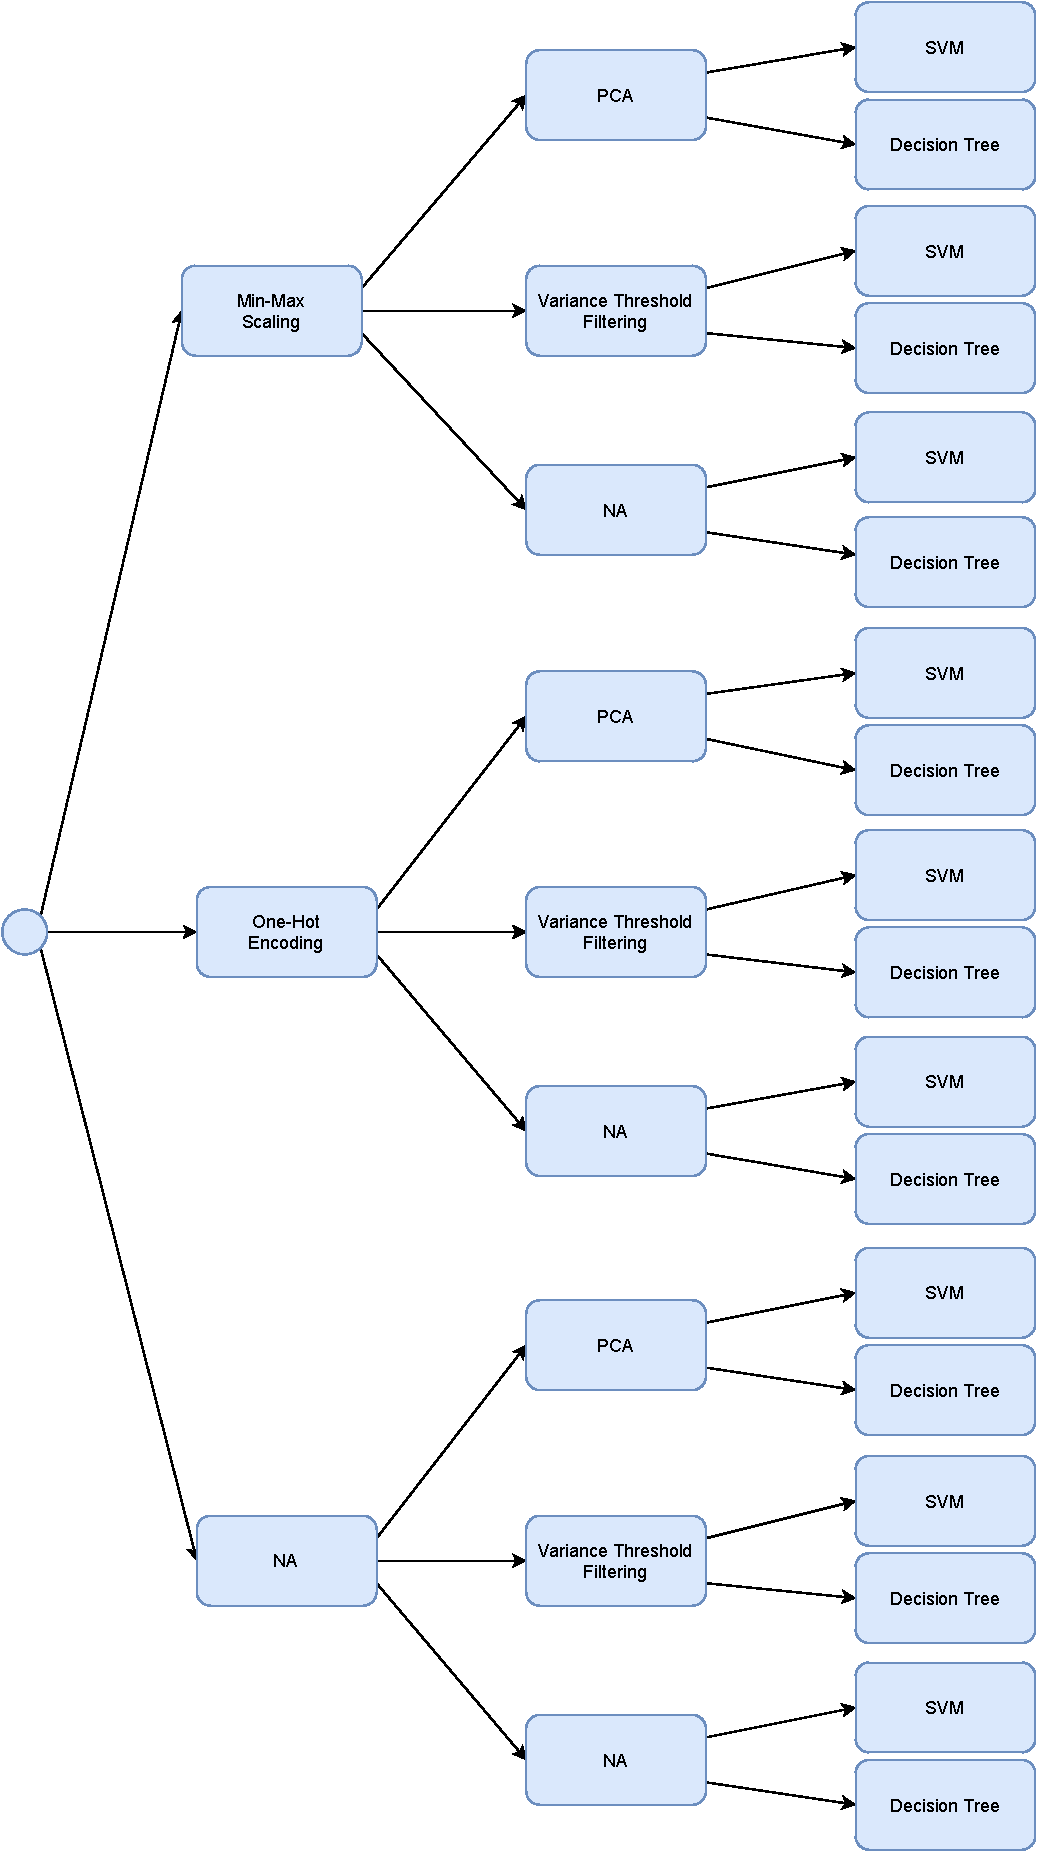
\includegraphics[height=\textheight,keepaspectratio]{gfx/Figures/Theory/ReinBoModelSelection.pdf}
    \caption{Simple visualization of the underlying concepts of the three layer ReinBo model selection candidate space.}
    \label{fig:theory:reinbo-model-selection}
\end{figure}
Because of the tree-like structure of this optimization space, a hierarchical Reinforcement Learning approach is trained during the optimization.
With learning about suitable pipeline component choices, it can act as an optimizer for model selection.\newline
After the Reinforcement Learning model has selected up to three pipeline components, the possible parametrization of each component is examined.
From the possible parametrization of each selected component a model configuration space can be induced.
Therewith, based on a completed model selection, the overall optimization space is once more transformed, but now to a space representing possible model configurations for the constructed pipeline.
Each leaf node of the tree structure has such a small model configuration space.\newline
Once the Reinforcement learning model performed the action of selecting a component from the last hierarchical layer and it reaches such a leaf node, Bayesian optimization is conducted in the model configuration space of this leaf.
The evaluation result of the best candidate of this optimization run is given as a reward to the Reinforcement Learning model such that it can update its policy.
Afterwards, in next iteration the Reinforcement Learning model starts once again in the root node and has to select pipeline components based on the policy and this is repeated until the optimization budget ist spent.\newline
Because Bayesian optimization is not very effective for high dimensional spaces, it is a suitable approach to not running a Bayesian optimization on the complete candidate space as an optimization approach.
Instead the model selection is performed by another optimizer and only a small portion of the model configuration space is the input for a Bayesian optimization run, which includes only the hyperparameter of the selected components.
The dimensionality is reduced to a great degree and Bayesian optimization will be more successful.\newline
But this improvements regarding the Bayesian optimization and the inclusion of a Reinforcement Learning model as an additional optimizer, does not extend the set of problem classes where this approach can be superior drastically, because there is still a big amount of problem classes where the Bayesian optimization method itself is not suitable.


The advantages of performing the AutoML optimization in several phases on transformed optimization spaces was further examined by~\textcite{Quemy-Two-Stage-Optimization}.
Besides the opportunity to compensate one less suitable optimization approach with another possibly better suited optimizer mentioned before, in this publication additionally was stated, that if the optimization space is transformed into two or more smaller sub-spaces, the overall optimization process can be sped up.
There, a two-stage optimization transformation was applied, alike ReinBo separating model configuration and model selection.
Although, this approach is not as limited to a mandatory pipeline topology as ReinBo, with the constraint of three components at most and only one of each type, and is able to construct pipelines in a more unrestricted fashion as a directed acyclic graph.
To create an optimization space of all valid pipeline graphs, all pipeline components have specifications of their input and output datatypes and can only be connected to another component node, if the output types of one node match the input types of another node.\newline
In the formal descriptions of this approach, no certain optimization algorithm is specified.
For this framework any optimization algorithm could be applied for either phase or the same one for both phases as well.
Instead, the publication focusses on the allocation of the optimization budget, in their case a time budget $T$, between the two phases.
The following allocation policies were defined:
\begin{itemize}
    \item \textit{Split policy}: $T$ is split into pre-defined phase allocations $T_1$ and $T_2$. $T_1$ is completely spent onto model selection and afterwards $T_2$ is spent as a whole as well.
    \item \textit{Iterative policy}: A very short time period $t << T$ is set and it will be alternated iteratively between the two phases, where each phase has $t$ as a budget in one iteration, until $T$ is spent.
    \item \textit{Adaptive policy}: This policy is an extension of the Iterative policy but here the $t$ is not fix but is adaptive to the achievements of the optimization in each phase.
    Therefore there is a $t_1$ and a $t_2$ for the corresponding phase.
    If in one iteration the evaluation score increases during the optimization of the active phase $i$, $t_i$ is doubled.
    In return, if the phase $i$ did not increase the evaluation score during its last two active iterations, $t_i$ is halved.
    \item \textit{Joint policy}: Here, no separation into different optimization phases takes place and model selection and model configuration is performed in a joint search space.
    Hence, it can spend $T$ completely.
\end{itemize}


Monte-Carlo simulations as a heuristic for a graph search, as explained in~\ref{sec:theory:optimization:search}, are the basis of graph search algorithm named \textit{Monte-Carlo tree search}(MCTS).
In this search algorithm the task of selecting the next child node of a tree node for expansion as an arm of an bandit problem.
With this approach, a ballance between exploring more unevaluated areas of the tree and exploiting sub-trees which have already shown promising scores can be achieved.
The Monte-Carlo tree search formalization \textit{UCT}(Upper Confidence bound applied to Trees)~\cite{Kocsis-UCT}.
Child nodes are selected with the following formula: $\underset{i}{\textrm{arg max}} \left( \mu_i + \sqrt{\frac{2 \cdot \textrm{log}(c)}{n_i}} \right)$, where $\mu_i$ is the overall sampled score of the subtree below node $i$ as an average, $n_i$ is the amount of times the sub-tree below $i$ was sampled and $n$ is the amount of overall iterations so far.\newline
MCTS will be exemplified in more detail in the next chapter but it is picked up here, since it is the basis for heuristic graph search based AutoML approach called \textit{Mosaic}~\cite{Rakotoarison-Mosaic}, which utilizes a multi-stage optimization method as well.
Here, the tree, which MCTS searches, is modelled as a transformation of the optimization space into a model selection space.
The first $k$ layers of the search tree are representing $k$ possible types of pipeline components, for example pre-processing methods or machine learning models, which have their corresponding $i \in [1,k]$ index in the resulting pipeline.
These pipelines are only linear and not generalized to any form of directed acyclic graph as in the prior related works approach.
In each of the first $k$ layers one component of each type is selected.
Therewith, this approach has a comparable tree structure to ReinBo but is more flexible regarding the length of the pipeline.\newline
After the model selection for a pipeline is concluded, the $k$ components of the pipeline need a configuration.
Thus, the continuous model configuration space that remains of the initial optimization space after the discrete model selection space has been covered with the search tree, is transformed into a sole model configuration space for the selected pipeline, which is embedded in the corresponding leaf node of the selected pipeline at the bottom of the $k$ model selection layers.
Similar to ReinBo, in each leaf node will a surrogate model $f_s$ of the expected evaluation score at any point of the optimization space for configuring the pipeline represented by the leaf be constructed and the optimization is based on this surrogate in the form of Bayesian optimization.


Mosaic and ReinBo have two remaining drawbacks:
\begin{itemize}
    \item They can only create pipelines of a fixed length and are without further extensions not capable of constructing more sophisticated non-linear pipeline, which limit the final pipeline potential for some datasets.
    \item Hyperparameter optimization in the second phase after the model selection is only performed with a single optimization method, namely Bayesian optimization, and is therefore limited by the capabilities of this method.
    But as outlined before with the aid of the No-Free-Lunch theorems, it is possible to improve the set of problem classes, for which an AutoML approach is superior by utilizing more than one optimization algorithm, if it is possible to automatically detect and exploit the most suitable optimizer for a problem class.
\end{itemize}
The approach of this thesis is similar to the principal of Mosaic and ReinBo but tries to overcome these two drawbacks.
In the following chapter, the functional principles of the approach of this thesis are explained in detail as well the strategies for both improvements.
